 \documentclass[12pt,a4paper]{article}

\usepackage{graphicx}% Include figure files
\usepackage{dcolumn}% Align table columns on decimal point
\usepackage{bm}% bold math
%\usepackage{hyperref}% add hypertext capabilities
%\usepackage[mathlines]{lineno}% Enable numbering of text and display math
%\linenumbers\relax % Commence numbering lines

%\usepackage[showframe,%Uncomment any one of the following lines to test 
%%scale=0.7, marginratio={1:1, 2:3}, ignoreall,% default settings
%%text={7in,10in},centering,
%%margin=1.5in,
%%total={6.5in,8.75in}, top=1.2in, left=0.9in, includefoot,
%%height=10in,a5paper,hmargin={3cm,0.8in},
%]{geometry}

\usepackage{multicol}%Para hacer varias columnas
\usepackage{multicol,caption}
\usepackage{multirow}
\usepackage{cancel}
\usepackage{hyperref}
\hypersetup{
    colorlinks=true,
    linkcolor=blue,
    filecolor=magenta,      
    urlcolor=cyan,
}

\setlength{\topmargin}{-1.0in}
\setlength{\oddsidemargin}{-0.3pc}
\setlength{\evensidemargin}{-0.3pc}
\setlength{\textwidth}{6.75in}
\setlength{\textheight}{9.5in}
\setlength{\parskip}{0.5pc}

\usepackage[utf8]{inputenc}
\usepackage{expl3,xparse,xcoffins,titling,kantlipsum}
\usepackage{graphicx}
\usepackage{xcolor} 
\usepackage{siunitx}

\usepackage{nopageno}
\usepackage{lettrine}
\usepackage{caption}
\renewcommand{\figurename}{Figura}
\usepackage{float}
\renewcommand\refname{Bibliograf\'ia}
\usepackage{amssymb}
\usepackage{amsmath}
\usepackage[rightcaption]{sidecap}
\usepackage[spanish]{babel}

\providecommand{\abs}[1]{\lvert#1\rvert}
\providecommand{\norm}[1]{\lVert#1\rVert}
\newcommand{\dbar}{\mathchar'26\mkern-12mu d}

\usepackage{mathtools}
\DeclarePairedDelimiter\bra{\langle}{\rvert}
\DeclarePairedDelimiter\ket{\lvert}{\rangle}
\DeclarePairedDelimiterX\braket[2]{\langle}{\rangle}{#1 \delimsize\vert #2}

% CABECERA Y PIE DE PÁGINA %%%%%
\usepackage{fancyhdr}
\pagestyle{fancy}
\fancyhf{}
\spanishdecimal{.}

\begin{document}

Macías Márquez Misael Iván

\begin{enumerate}



%%%1%%%



\item La línea de mundo de una partícula está descrita por las siguientes ecuaciones paramétricas

\begin{equation*}
    t(\lambda) = a \sinh{(\lambda/a)} \hspace{2cm} x(\lambda) = a \cosh{(\lambda/a)}
\end{equation*}

en donde $\lambda$ es un parámetro y $a$ es una constante real. Describa el movimiento y calcule las componentes de la cuadri-velocidad y de la cuadri-aceleración. ¿Qué relación hay entre el parámetro $\lambda$ y el tiempo propio de la partícula?

\textbf{Sol:}


Por definición de la cuadri-velocidad:

\begin{equation*}
    u ^{\mu} = \left(\frac{\partial t}{\partial \tau}, \frac{\partial x}{\partial \tau}\right) = \left(\frac{\partial t}{\partial \lambda} \frac{\partial \lambda}{\partial \tau},\frac{\partial x}{\partial \lambda} \frac{\partial \lambda}{\partial \tau}\right)
\end{equation*}

\begin{equation*}
    =\left(\cosh{\frac{\lambda}{a}}\frac{\partial \lambda}{\partial \tau}, \sinh{\frac{\lambda}{a}}\frac{\partial \lambda}{\partial \tau}\right) = \frac{\partial \lambda}{\partial \tau} \left(\cosh{\frac{\lambda}{a}},\sinh{\frac{\lambda}{a}}\right)
\end{equation*}

\begin{equation*}
    =\frac{\partial \lambda}{\partial \tau}\frac{1}{\cosh{\frac{\lambda}{a}}} \left(1,\tanh{\frac{\lambda}{a}}\right)
\end{equation*}

con $\tau$ el tiempo propio, por lo anterior y como $u^{\mu}=\gamma(1,\overline{v})$, entonces $\gamma = \frac{\partial \lambda}{\partial \tau}\frac{1}{\cosh{\frac{\lambda}{a}}}$ y $\overline{v} = \tanh{\frac{\lambda}{a}}$.

Por definición de la cuadri-aceleración:

\begin{equation*}
    \frac{d u^{\mu}}{d \tau} = \frac{d}{d \tau} \left( \left(\frac{\partial \lambda}{\partial \tau}\frac{1}{\cosh{\frac{\lambda}{a}}},\frac{\partial \lambda}{\partial \tau}\frac{1}{\cosh{\frac{\lambda}{a}}}\tanh{\frac{\lambda}{a}}\right)\right)
\end{equation*}

\begin{equation*}
    =
\end{equation*}

\begin{equation*}
    \hspace{-4cm}=\left(\frac{1}{\cosh{\lambda/a}}\frac{\partial^2 \lambda}{\partial \tau^2} - \frac{\partial^2 \lambda}{\partial \tau^2} \frac{\tanh{\lambda/2}\text{ sech }\lambda/2}{a},(\frac{\partial \lambda}{\partial \tau})^2\frac{1}{\cosh{\frac{\lambda}{a}}}  \frac{\text{ sech}^2 \lambda/a}{a} +\left(\frac{1}{\cosh{\lambda/a}}\frac{\partial^2 \lambda}{\partial \tau^2} - \frac{\partial^2 \lambda}{\partial \tau^2} \frac{\tanh{\lambda/2}\text{ sech }\lambda/2}{a}\right) \tanh{\frac{\lambda}{a}} \right)
\end{equation*}







%%%2%%%



\item Demuestre que la cuadri-aceleración de un observador tiene solo tres componentes independientes, escriba la relación entre estas tres componentes y la aceleración que mediría un observador en una descripción newtoniana.

\textbf{Sol:}

Para una trayectoria parametrizada por $x(t)$, $y(t)$, $z(t)$, la cuadri-velocidad es:

\begin{equation*}
    u^{\mu} = \frac{d x^{\mu}}{d\tau} = \left(\frac{\partial t}{\partial \tau},\frac{\partial x}{\partial \tau},\frac{\partial y}{\partial \tau},\frac{\partial z}{\partial \tau}\right)
\end{equation*}

\begin{equation*}
    =\left(\frac{\partial t}{\partial \tau}, \frac{\partial x}{\partial t} \frac{\partial t}{\partial \tau},\frac{\partial y}{\partial t} \frac{\partial t}{\partial \tau},\frac{\partial z}{\partial t} \frac{\partial t}{ \partial \tau}\right)
\end{equation*}

y por definición la cuadri-aceleración es:

\begin{equation*}
    a^{\mu} = \frac{d u^{\mu}}{d \tau} = \left(\frac{\partial^2 t}{\partial \tau^2},\frac{\partial}{\partial \tau}(  \frac{\partial x}{\partial t} \frac{\partial t}{\partial \tau}),\frac{\partial}{\partial \tau}(\frac{\partial y}{\partial t} \frac{\partial t}{\partial \tau}),\frac{\partial}{\partial \tau}(\frac{\partial z}{\partial t} \frac{\partial t}{\partial \tau}) \right)
\end{equation*}

\begin{equation*}
    =\left(\frac{\partial^2 t}{\partial \tau^2},\frac{\partial^2 x}{\partial t^2}\frac{\partial t}{\partial \tau}+ 2 \frac{\partial x}{\partial t} \frac{\partial^2 t }{\partial \tau^2},\frac{\partial^2 y}{\partial t^2}\frac{\partial t}{\partial \tau}+ 2 \frac{\partial y}{\partial t} \frac{\partial^2 t }{\partial \tau^2},\frac{\partial^2 z}{\partial t^2}\frac{\partial t}{\partial \tau}+ 2 \frac{\partial z}{\partial t} \frac{\partial^2 t }{\partial \tau^2}\right)
\end{equation*}

para una descripción newtoniana se tiene:

\begin{equation*}
    v=\left(\frac{\partial x}{\partial t},\frac{\partial y}{\partial t} ,\frac{\partial z}{\partial t}\right) = (v_1,v_2,v_3) \hspace{1cm}a=\left(\frac{\partial^2 x}{\partial t^2},\frac{\partial^2 y}{\partial t^2} ,\frac{\partial^2 z}{\partial t^2}\right) = (a_1,a_2,a_3)
\end{equation*}

por lo que la cuadri-aceleración se puede escribir como:

\begin{equation*}
    a^{\mu}=\left(\frac{\partial^2 t}{\partial \tau^2},a_1\frac{\partial t}{\partial \tau}+ 2 v_1 \frac{\partial^2 t }{\partial \tau^2},a_2\frac{\partial t}{\partial \tau}+ 2 v_2 \frac{\partial^2 t }{\partial \tau^2},a_3\frac{\partial t}{\partial \tau}+ 2 v_3 \frac{\partial^2 t }{\partial \tau^2}\right)
\end{equation*}



%%%3%%%



\item La trayectoria de una partícula está descrita por

\begin{equation*}
    x(t) =b\sin{(\omega t)} \hspace{0.5cm} y(t) = b \sin{(\omega t)} \hspace{0.5cm} z(t) = at
\end{equation*}

en el espacio tridimensional. Describa el movimiento y calcula las componentes de la cuadri-velocidad. Dibuje la trayectoria en un diagrama de espacio-tiempo.

\textbf{Sol:}

El movimiento en el plano $xy$ es la recta identidad pero cortada desde $-b$ hasta $b$ y como en el eje $z$ también se tiene una recta, en el espacio $xyz$ es una especie de zigzag que  va en la dirección de $z$ y que oscila entre $-b$ y $b$.

\begin{equation*}
    u^{\mu}= \left(\frac{\partial t}{\partial \tau}, \frac{\partial x}{\partial \tau},\frac{\partial y}{\partial \tau}, \frac{\partial z}{\partial \tau}\right) = \left(\frac{\partial t}{\partial \tau}, \frac{\partial x}{\partial t}\frac{\partial t}{\partial \tau},\frac{\partial y}{\partial t}\frac{\partial t}{\partial \tau}, \frac{\partial z}{\partial t}\frac{\partial t}{\partial \tau}\right)
\end{equation*}

\begin{equation*}
    =\frac{\partial t}{\partial \tau}\left(1, \frac{\partial x}{\partial t},\frac{\partial y}{\partial t}, \frac{\partial z}{\partial t}\right)=\frac{\partial t}{\partial \tau}\left(1, \omega b \cos{\omega t},\omega b \cos{\omega t}, a\right)
\end{equation*}

\begin{equation*}
    =\gamma\omega b\left(\frac{1}{\omega b}, \cos{\omega t},\cos{\omega t}, \frac{a}{\omega b}\right)
\end{equation*}

\newpage

\begin{figure}[h!]
    \centering
    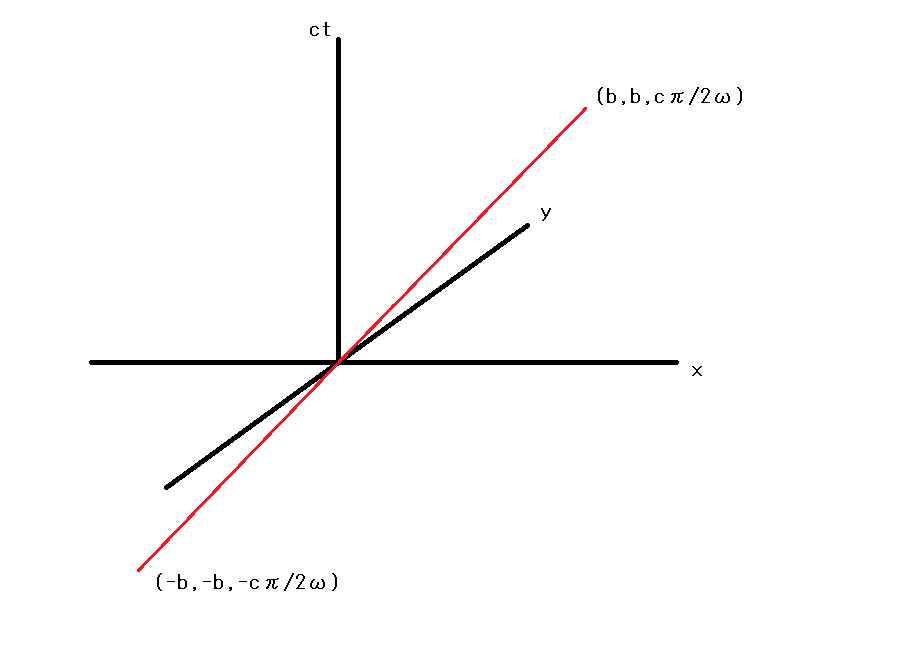
\includegraphics[scale=0.4]{xy rela.png}
\end{figure}

\begin{figure}[h!]
    \centering
    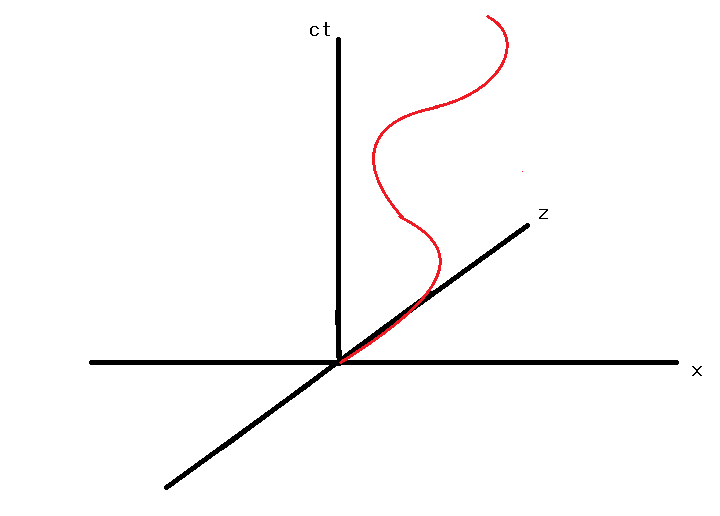
\includegraphics[scale=0.4]{xz rela.png}
\end{figure}

%$\vspace{6.5cm}$

y para $yz$ es análogo.




%%%4%%%



\item Un haz de luz se emite formando un ángulo $\phi'$ con respecto al eje $x'$ del sistema de referencia de un cohete en movimiento. Muestre que el ángulo que tiene la dirección de este haz con respecto al eje $x$ del sistema de referencia del laboratorio está dado (en unidades geométricas) por la ecuación:

\begin{equation*}
    \cos{\phi} = \frac{\cos{\phi'} + v}{1+v \cos{\phi'}}
\end{equation*}

con $v$ la velocidad relativa entre sistemas en la configuración estándar.

\textbf{Sol:}
No encontré la forma exacta pero sí algo parecido.

Sabemos que $\tan{\alpha}=v$, y del diagrama se puede ver que $\alpha=\phi -\phi'$ por lo que $\tan{\phi-\phi'}= v$ y usando la formula para la suma de ángulos en la tangente:

\begin{equation*}
    v=\tan{\phi-\phi'} =\frac{\tan{\phi}-\tan{\phi'}}{1-\tan{\phi}\tan{\phi'}}
\end{equation*}

\begin{equation*}
    (1-\tan{\phi}\tan{\phi'})(v)=\tan{\phi}-\tan{\phi'}
\end{equation*}

\begin{equation*}
    v-\tan{\phi}\tan{\phi'}v=\tan{\phi}-\tan{\phi'}
\end{equation*}

\begin{equation*}
    v+\tan{\phi'}=\tan{\phi}+\tan{\phi}\tan{\phi'}v
\end{equation*}

\begin{equation*}
    v+\tan{\phi'}=\tan{\phi}(1+v\tan{\phi'})
\end{equation*}


\begin{equation*}
    \tan{\phi}=\frac{v+\tan{\phi'}}{1+v\tan{\phi'}}
\end{equation*}






\begin{figure}[h!]
    \centering
    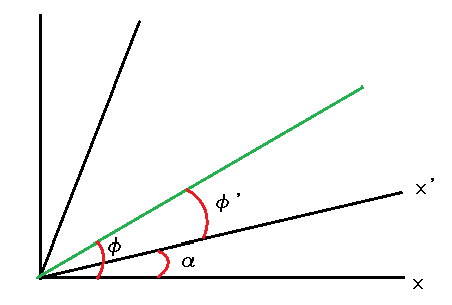
\includegraphics[scale=0.6]{diagrama.png}
\end{figure}



%%%5%%%




\item Demuestre que cualquier tensor covariante de tipo $(0,2)$ puede escribirse como la suma de un tensor simétrico y otro antisimétrico.

\textbf{Sol:}

Sea $T_{\alpha \beta}$ un tensor covariante de tipo $(0,2)$ entonces se cumple que:

\begin{equation*}
    T_{\alpha \beta} = \frac{(T_{\alpha \beta} + T_{ \beta \alpha}) +(T_{\alpha \beta} - T_{\beta \alpha})}{2} = \frac{T_{\alpha \beta} + T_{\beta \alpha}}{2} + \frac{T_{\alpha \beta} - T_{\beta \alpha}}{2}
\end{equation*}

pero notemos que $A_{\alpha \beta}=\frac{T_{\alpha \beta}+ T_{\beta \alpha}}{2}$ es simétrico ya que $A_{\alpha \beta} = A_{\beta \alpha}$ y $B_{\alpha \beta} = \frac{T_{\alpha \beta} - T_{\beta \alpha}}{2}$ es antisimetrico ya que $B_{\alpha  \beta} = - B_{\beta \alpha}$.

Por lo tanto el tensor covariante $T_{\alpha \beta}$ de tipo $(0,2)$ se puede escribir como:

\begin{equation*}
    T_{\alpha \beta} = A_{\alpha \beta} + B_{\alpha \beta}
\end{equation*}

donde $A_{\alpha \beta}$ es un tensor simétrico y $B_{\alpha \beta}$ es antisimetrico.
    
    
\end{enumerate}

\end{document}